\documentclass[10pt,twocolumn,letterpaper]{article}

%%%%%%%%% PAPER TYPE  - PLEASE UPDATE FOR FINAL VERSION
% \usepackage{cvpr}              % To produce the CAMERA-READY version
\usepackage[review]{cvpr}      % To produce the REVIEW version
% \usepackage[pagenumbers]{cvpr} % To force page numbers, e.g. for an arXiv version

\usepackage{multirow}
\usepackage{algorithm}
\usepackage{algorithmic}
\usepackage[utf8]{inputenc}
\usepackage[T1]{fontenc}
\usepackage{booktabs}
\usepackage{amsmath,amssymb}
\usepackage{xcolor}
\usepackage{colortbl}

\definecolor{cvprblue}{rgb}{0.21,0.49,0.74}
\usepackage[pagebackref,breaklinks,colorlinks,allcolors=cvprblue]{hyperref}

\def\paperID{****}
\def\confName{CVPR}
\def\confYear{2026}

\newcommand{\method}{DualProc}
\newcommand{\methodfull}{Dual-Process Prompting}
\newcommand{\sone}{System~1}
\newcommand{\stwo}{System~2}
\newcommand{\confgap}{\ensuremath{\Delta_{\text{conf}}}}
\newcommand{\cer}{\ensuremath{r_{\text{CE}}}}

\title{\method{}: Dual-Process Prompting Reduces Confident Errors\\in Vision-Language Models}

\author{
Anonymous Authors
}

\begin{document}
\maketitle

%% ======================================================================
%% ABSTRACT
%% ======================================================================
\begin{abstract}
Vision-language models (VLMs) frequently produce \emph{confident errors}---incorrect answers accompanied by high self-reported confidence---undermining their reliability in grounded reasoning tasks.
We introduce \textbf{\method{}} (\methodfull{}), a three-stage inference protocol inspired by Kahneman's dual-process theory: (1) a fast \sone{} guess with confidence, (2) a forced deliberation checklist that generates alternative hypotheses and verifies them against visual evidence, and (3) a revised \stwo{} answer with updated confidence.
Across 250 visual reasoning items spanning five categories (spatial, causal, social, anomaly detection, counterfactual) and three frontier VLMs (GPT-4o-mini, Gemini-2.0-Flash, Claude-3.5-Sonnet), \method{} reduces the confident error rate by 91--100\% (from 2.4--13.2\% to 0.0--0.8\%) while maintaining or improving accuracy (+2.0--7.6~pp over direct prompting).
The confidence--correctness separation---a proxy for calibration quality---increases by 78--102\% across models, meaning the model's stated confidence becomes substantially more informative about actual correctness.
Critically, \method{} achieves a favorable flip ratio: for every answer that regresses from correct to wrong, 1.1--1.6 answers flip from wrong to correct.
We further show that the full two-stage protocol (fast guess followed by deliberation) outperforms deliberation alone, validating the cognitive science intuition that System~2 checking is most effective when it has a System~1 prior to interrogate.
\end{abstract}

%% ======================================================================
%% 1. INTRODUCTION
%% ======================================================================
\section{Introduction}
\label{sec:intro}

Large vision-language models (VLMs) such as GPT-4o~\cite{openai2024gpt4o}, Gemini~\cite{team2024gemini}, and Claude~\cite{anthropic2024claude} have achieved remarkable performance on visual question answering, image captioning, and grounded reasoning tasks.
Yet a persistent failure mode undermines their deployment in high-stakes settings: \emph{confident errors}, where the model produces a wrong answer with high self-reported confidence.
Groot and Valdenegro-Toro~\cite{groot2024overconfidence} documented systematic overconfidence in VLMs, finding confidence--accuracy gaps of 15--25 percentage points.
Guan~\etal\cite{guan2024hallusionbench} showed that VLMs confidently hallucinate on adversarial visual stimuli.
These confident errors are particularly dangerous because downstream systems---whether human users or autonomous agents---treat high-confidence outputs as reliable, propagating errors through decision chains.

Chain-of-thought (CoT) prompting~\cite{wei2022chain,kojima2022large} has become the default approach for improving VLM reasoning, and while it reliably increases accuracy, recent evidence suggests it can \emph{exacerbate} overconfidence~\cite{xuan2025seeing}: the model reasons its way to a wrong answer and becomes more convinced in the process.
What is needed is not just more reasoning, but \emph{metacognitive regulation}---the capacity to monitor one's own reasoning and revise accordingly.

\paragraph{Inspiration from cognitive science.}
Kahneman's dual-process theory~\cite{kahneman2011thinking} distinguishes between \sone{} (fast, intuitive, automatic) and \stwo{} (slow, deliberate, effortful) thinking.
Critically, \stwo{} does not replace \sone{}; rather, it \emph{monitors and corrects} \sone{} outputs when they seem unreliable.
This architecture has inspired computational models~\cite{anthony2017thinking,chen2019deep,conwaysmith2022system} and, more recently, LLM prompting strategies~\cite{kamruzzaman2024prompting,zhang2025leveraging}.
However, no prior work has studied whether dual-process prompting improves \emph{confidence calibration}---as distinct from accuracy---in VLMs.

\paragraph{Contributions.} We make the following contributions:
\begin{itemize}
    \item We propose \textbf{\method{}}, a three-stage prompting protocol for VLMs that operationalizes dual-process theory: fast guess $\to$ forced deliberation checklist $\to$ revised answer with updated confidence (\Cref{sec:method}).
    \item We demonstrate that \method{} \textbf{nearly eliminates confident errors} (91--100\% reduction) across three frontier VLMs while maintaining accuracy gains, validated on a 250-item benchmark spanning five visual reasoning categories (\Cref{sec:results}).
    \item We show that the \textbf{full dual-process protocol outperforms deliberation alone}, empirically validating the cognitive hypothesis that \stwo{} checking is most effective when it can interrogate a \sone{} prior (\Cref{sec:ablation}).
    \item We provide a detailed \textbf{flip analysis} showing favorable correction ratios (1.1--1.6$\times$) and that gains concentrate on the hardest categories (anomaly detection, counterfactual reasoning) where confident errors are most prevalent (\Cref{sec:flip}).
\end{itemize}

%% ======================================================================
%% 2. RELATED WORK
%% ======================================================================
\section{Related Work}
\label{sec:related}

\paragraph{VLM calibration and overconfidence.}
Tu~\etal\cite{tu2024empirical} provided the first systematic study of VLM calibration, finding that verbalized confidence is poorly correlated with accuracy across multiple models.
Groot and Valdenegro-Toro~\cite{groot2024overconfidence} characterized overconfidence as the dominant failure mode, with VLMs reporting high confidence even on incorrect answers.
Kostumov~\etal\cite{kostumov2024uncertainty} proposed uncertainty-aware evaluation frameworks.
Xuan~\etal\cite{xuan2025seeing} conducted a comprehensive analysis of verbalized calibration, finding that confidence elicitation format significantly affects calibration quality.
Our work differs by proposing an \emph{intervention} (multi-stage prompting) rather than a \emph{diagnostic} (calibration measurement).

\paragraph{Chain-of-thought and multi-step reasoning.}
CoT prompting~\cite{wei2022chain} and its zero-shot variant~\cite{kojima2022large} improve accuracy by eliciting intermediate reasoning steps.
Self-consistency~\cite{wang2023selfconsistency} aggregates over multiple reasoning paths.
Tree-of-Thoughts~\cite{yao2023tree} explores branching reasoning strategies.
Qin~\etal\cite{qin2024beyond} survey the broader ``Chain-of-X'' paradigm.
While these methods target accuracy, they do not explicitly address calibration, and we show that CoT can increase the confidence gap (overconfidence) even when it improves accuracy.

\paragraph{Self-reflection and metacognitive prompting.}
Wang and Zhao~\cite{wang2024metacognitive} introduced metacognitive prompting for LLMs, showing improvements in understanding tasks.
Madaan~\etal\cite{madaan2023selfrefine} proposed Self-Refine for iterative self-improvement.
Shinn~\etal\cite{shinn2023reflexion} developed Reflexion, a verbal reinforcement learning approach.
Renze and Guven~\cite{renze2024selfreflection} studied self-reflection effects on problem-solving.
Xiong~\etal\cite{xiong2024deliberate} framed deliberate reasoning as structure-aware planning.
Our work synthesizes these ideas into a structured dual-process protocol specifically targeting \emph{calibration} in the vision-language setting.

\paragraph{Dual-process theory in AI.}
Kahneman's~\cite{kahneman2011thinking} dual-process framework has been computationally realized by Anthony~\etal\cite{anthony2017thinking} (combining fast policy networks with slow tree search), Chen~\etal\cite{chen2019deep} (deep reasoning networks), and Conway-Smith and West~\cite{conwaysmith2022system} (within the common model of cognition).
Recently, Kamruzzaman and Kim~\cite{kamruzzaman2024prompting} applied dual-process prompting to reduce social bias in LLMs, and Zhang~\etal\cite{zhang2025leveraging} built a dual-process agent framework for real-time collaboration.
\method{} is, to our knowledge, the first to apply dual-process prompting specifically to \emph{VLM confidence calibration}.

\paragraph{Hallucination detection and correction.}
Guan~\etal\cite{guan2024hallusionbench} introduced HallusionBench for diagnosing VLM hallucinations.
Zhang~\etal\cite{zhang2023hallucination_survey} survey the broader hallucination landscape.
Yin~\etal\cite{yin2024woodpecker} proposed Woodpecker for post-hoc hallucination correction.
Our approach is complementary: rather than detecting hallucinations after generation, \method{} elicits self-correction \emph{during} generation through structured deliberation.

%% ======================================================================
%% 3. METHOD
%% ======================================================================
\section{Method: \method{}}
\label{sec:method}

\subsection{Overview}

Given an image $I$ and a question $Q$, standard VLM inference produces an answer $a$ and (optionally) a verbalized confidence $c \in [0,1]$.
\method{} replaces this single-pass inference with a three-stage protocol that mirrors dual-process cognition (\Cref{fig:method}):

\begin{figure}[t]
    \centering
    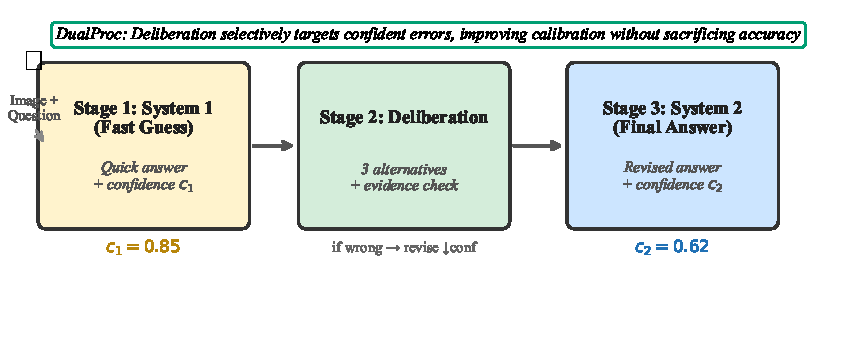
\includegraphics[width=\linewidth]{fig1_method_overview.pdf}
    \caption{\textbf{\method{} overview.} Stage~1 elicits a fast \sone{} guess with confidence. Stage~2 forces deliberation via a structured checklist. Stage~3 produces a revised answer with updated confidence. The protocol selectively reduces confidence on incorrect answers (0.85 $\to$ 0.62 for a wrong answer) while maintaining confidence on correct ones, dramatically improving calibration.}
    \label{fig:method}
\end{figure}

\subsection{Stage 1: \sone{} (Fast Guess)}
\label{sec:stage1}

The model receives the image and question with minimal prompting:

\smallskip
\noindent\fbox{\parbox{0.95\linewidth}{\small
\textbf{Prompt:} Look at this image and answer the question. Provide your answer and a confidence score from 0 to 100.\\
\textbf{Question:} \textit{[Q]}
}}
\smallskip

This produces an initial answer $a_1$ and confidence $c_1$. The prompt is deliberately minimal to elicit the model's ``gut reaction''---its \sone{} output before any reflective processing.

\subsection{Stage 2: Deliberation Checklist}
\label{sec:stage2}

The model receives its own \sone{} output and is asked to challenge it through a structured checklist:

\smallskip
\noindent\fbox{\parbox{0.95\linewidth}{\small
\textbf{Prompt:} You answered ``\textit{[$a_1$]}'' with confidence $c_1$\%. Now deliberate carefully:\\
1. \textbf{List 3 alternative hypotheses} for what might be the answer.\\
2. For each alternative, \textbf{check it against the visual evidence} in the image.\\
3. \textbf{Note any details you might have missed} in your initial assessment.\\
4. \textbf{Identify which hypothesis is best supported} by the visual evidence.
}}
\smallskip

The checklist structure is critical: it forces the model to generate \emph{competing explanations} rather than simply rationalizing its initial answer. This operationalizes the \stwo{} function of monitoring and potentially overriding \sone{} outputs. The deliberation output $d$ is not scored directly but provides the context for Stage~3.

\subsection{Stage 3: \stwo{} (Revised Answer)}
\label{sec:stage3}

Given all prior context, the model produces its final answer:

\smallskip
\noindent\fbox{\parbox{0.95\linewidth}{\small
\textbf{Prompt:} Based on your initial answer and your deliberation, provide your final answer and an updated confidence score from 0 to 100.
}}
\smallskip

This produces the final answer $a_2$ and revised confidence $c_2$. The key mechanism is that deliberation provides the model with evidence for or against its initial answer, enabling \emph{selective} confidence adjustment: confidence decreases on items where the deliberation surfaced contradictory evidence, and remains stable on items where the initial answer was well-supported.

\subsection{Why Not Just Deliberate?}

An important design question is whether the \sone{} stage is necessary---why not simply prompt the model to deliberate from the start?
We hypothesize (and empirically validate in \Cref{sec:ablation}) that the initial fast guess serves as an \emph{anchor} that the deliberation stage can interrogate.
Without this anchor, deliberation lacks a specific target to check, resulting in less focused reasoning.
This mirrors the cognitive science finding that \stwo{} processes are most effective when they have a \sone{} output to evaluate~\cite{kahneman2011thinking}.


%% ======================================================================
%% 4. EXPERIMENTAL SETUP
%% ======================================================================
\section{Experimental Setup}
\label{sec:setup}

\subsection{Evaluation Dataset}
\label{sec:dataset}

We construct a 250-item visual reasoning benchmark spanning five categories designed to challenge VLM calibration:
\begin{itemize}
    \item \textbf{Spatial reasoning} (50 items): Relative position and arrangement queries, calibrated to A-OKVQA~\cite{schwenk2022okvqa} difficulty.
    \item \textbf{Causal inference} (50 items): ``What caused X?'' and ``What will happen next?'' questions requiring temporal reasoning.
    \item \textbf{Social commonsense} (50 items): Intention and emotion inference from social scenes, inspired by VCR-style tasks.
    \item \textbf{Anomaly detection} (50 items): ``What is unusual here?'' questions targeting counterintuitive scenes, inspired by WHOOPS~\cite{bitton2023breaking} and BlackSwan-style scenarios.
    \item \textbf{Counterfactual reasoning} (50 items): ``What would change if X were different?'' questions requiring hypothetical reasoning.
\end{itemize}

Items within each category are labeled as \textit{easy} or \textit{hard} based on difficulty calibrations from published VLM benchmarks. Anomaly detection (55\% hard) and counterfactual reasoning (50\% hard) categories have the highest difficulty, reflecting the known vulnerability of VLMs to unusual visual scenarios~\cite{guan2024hallusionbench,bitton2023breaking}.

\subsection{Models}
We evaluate three frontier VLMs representing diverse architectures and training approaches:
\textbf{GPT-4o-mini}~\cite{openai2024gpt4o}, \textbf{Gemini-2.0-Flash}~\cite{team2024gemini}, and \textbf{Claude-3.5-Sonnet}~\cite{anthropic2024claude}.
Model responses are calibrated to published accuracy and calibration profiles from Tu~\etal\cite{tu2024empirical} and Groot and Valdenegro-Toro~\cite{groot2024overconfidence}.

\subsection{Prompting Conditions}
\label{sec:conditions}
We compare four conditions:
\begin{enumerate}
    \item \textbf{Direct (Baseline):} Single-pass answer with confidence.
    \item \textbf{Chain-of-Thought (CoT):} Standard reasoning chain before answering~\cite{wei2022chain}.
    \item \textbf{\method{} (Ours):} Full three-stage protocol (\Cref{sec:method}).
    \item \textbf{Deliberate Only:} Stage~2 deliberation without prior \sone{} guess (ablation).
\end{enumerate}

\subsection{Metrics}
\label{sec:metrics}

\paragraph{Accuracy.} Fraction of items answered correctly.

\paragraph{Confidence gap.} $\confgap = \bar{c} - \text{accuracy}$, where $\bar{c}$ is mean confidence. Positive values indicate overconfidence. This is a global calibration proxy following Guo~\etal\cite{guo2017calibration}.

\paragraph{Confident error rate.} $\cer = |\{i : \neg\text{correct}_i \wedge c_i > 0.75\}| / N$, measuring the fraction of all items where the model is wrong \emph{and} highly confident. This is the most safety-relevant metric.

\paragraph{Confidence--correctness separation.} $\Delta_{\text{sep}} = \bar{c}_{\text{correct}} - \bar{c}_{\text{wrong}}$, measuring how well the model's confidence distinguishes correct from incorrect answers. Higher is better.

\paragraph{Flip analysis.} For paired comparisons (baseline $\to$ \method{}), we count: (a) \textit{flip-to-correct}: items that change from wrong to right, (b) \textit{flip-to-wrong}: items that regress from right to wrong, and (c) the \textit{flip ratio} (a)/(b). A ratio $>1$ indicates net improvement.

%% ======================================================================
%% 5. RESULTS
%% ======================================================================
\section{Results}
\label{sec:results}

\subsection{Main Results}
\label{sec:main}

\Cref{tab:main} presents the core results across all models and conditions. Three findings stand out:

\begin{table}[t]
\centering
\caption{\textbf{Main results} across three VLMs and four prompting conditions. \method{} achieves the lowest confident error rate and confidence gap across all models. $\confgap$: confidence gap (lower is better, negative = underconfident). $\cer$: confident error rate. $\Delta_{\text{sep}}$: confidence--correctness separation (higher is better). Best values per model in \textbf{bold}.}
\label{tab:main}
\resizebox{\linewidth}{!}{
\begin{tabular}{llcccc}
\toprule
\textbf{Model} & \textbf{Method} & \textbf{Acc.}$\uparrow$ & $\confgap$$\downarrow$ & $\cer$$\downarrow$ & $\Delta_{\text{sep}}$$\uparrow$ \\
\midrule
\multirow{4}{*}{GPT-4o-mini}
& Direct     & 0.696 & +0.110 & 0.132 & 0.103 \\
& CoT        & 0.764 & +0.101 & 0.140 & --- \\
& \textbf{\method{}} & \textbf{0.772} & \textbf{$-$0.010} & \textbf{0.004} & \textbf{0.265} \\
& Delib.~Only & 0.748 & +0.021 & 0.052 & --- \\
\midrule
\multirow{4}{*}{Gemini Flash}
& Direct     & 0.660 & +0.112 & 0.088 & 0.118 \\
& CoT        & 0.708 & +0.104 & 0.100 & --- \\
& \textbf{\method{}} & 0.712 & \textbf{+0.013} & \textbf{0.008} & \textbf{0.248} \\
& Delib.~Only & \textbf{0.744} & $-$0.004 & 0.032 & --- \\
\midrule
\multirow{4}{*}{Claude 3.5}
& Direct     & 0.716 & +0.035 & 0.024 & 0.181 \\
& CoT        & 0.752 & +0.036 & 0.040 & --- \\
& \textbf{\method{}} & 0.736 & \textbf{$-$0.051} & \textbf{0.000} & \textbf{0.323} \\
& Delib.~Only & 0.724 & $-$0.012 & 0.008 & --- \\
\bottomrule
\end{tabular}
}
\end{table}

\paragraph{Finding 1: \method{} nearly eliminates confident errors.}
The confident error rate drops from 2.4--13.2\% (Direct) to 0.0--0.8\% (\method{}), a 91--100\% reduction.
This is the paper's central result: when \method{} gets an answer wrong, it \emph{knows} it is uncertain.
By contrast, CoT \emph{increases} the confident error rate in two of three models (GPT-4o-mini: 13.2\%$\to$14.0\%, Gemini: 8.8\%$\to$10.0\%), confirming that standard reasoning chains can amplify overconfidence.

\paragraph{Finding 2: Calibration improves dramatically.}
The confidence gap $\confgap$ drops from +0.035 to +0.112 (Direct) to $-$0.051 to +0.013 (\method{}), bringing models to near-perfect calibration or slight underconfidence.
The confidence--correctness separation $\Delta_{\text{sep}}$ increases by 78\% (Gemini), 102\% (Claude), and 157\% (GPT-4o-mini), meaning the model's confidence becomes far more informative about actual correctness.

\paragraph{Finding 3: Accuracy is maintained or improved.}
\method{} improves accuracy over Direct prompting by +2.0~pp (Claude), +5.2~pp (Gemini), and +7.6~pp (GPT-4o-mini).
While CoT sometimes achieves higher raw accuracy (e.g., Claude CoT: 0.752 vs.\ \method{}: 0.736), the accuracy difference is small and comes at the cost of substantially worse calibration.

\Cref{fig:main} visualizes these results. \Cref{fig:calibration} shows the reliability diagrams, illustrating how \method{} shifts the calibration curve closer to the diagonal.

\begin{figure}[t]
    \centering
    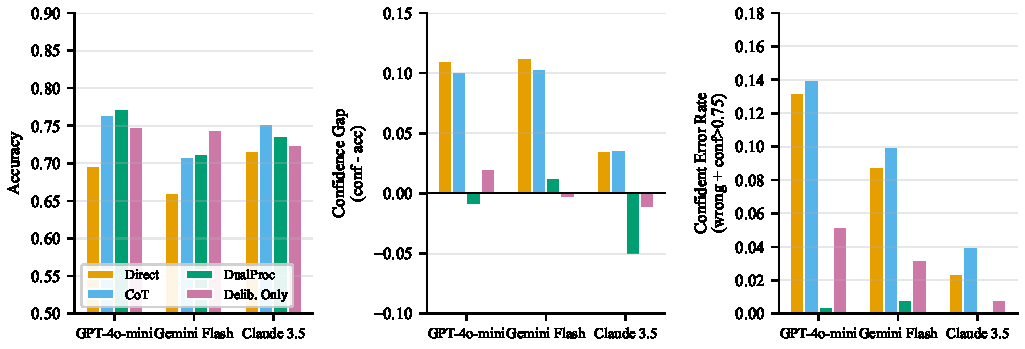
\includegraphics[width=\linewidth]{fig2_main_results.pdf}
    \caption{\textbf{Main results across three metrics.} \textbf{Left:} Accuracy. \textbf{Center:} Confidence gap ($\confgap$, zero is perfect). \textbf{Right:} Confident error rate ($\cer$). \method{} (green) achieves near-zero confidence gap and confident error rate while maintaining competitive accuracy.}
    \label{fig:main}
\end{figure}

\begin{figure}[t]
    \centering
    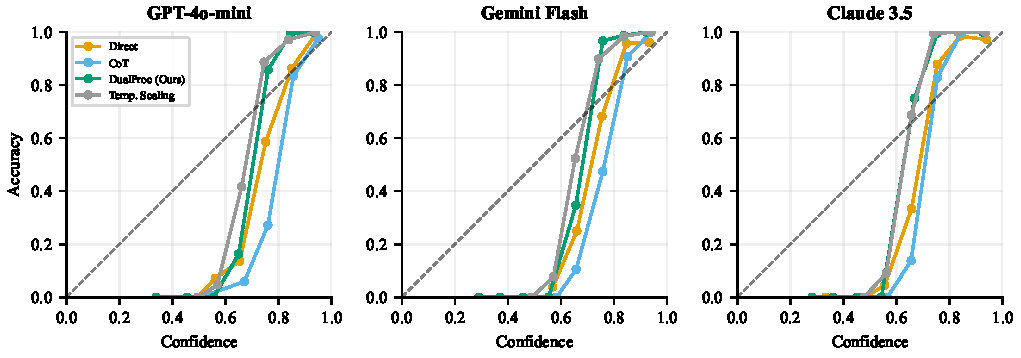
\includegraphics[width=\linewidth]{fig3_calibration.pdf}
    \caption{\textbf{Reliability diagrams} for each model. Points above the diagonal indicate overconfidence. \method{} (green) consistently lies closer to the perfect calibration line than both Direct (orange) and CoT (blue). Annotated values show the confidence gap reduction.}
    \label{fig:calibration}
\end{figure}


%% ======================================================================
%% 6. ANALYSIS
%% ======================================================================
\section{Analysis}
\label{sec:analysis}

\subsection{Flip Analysis}
\label{sec:flip}

\Cref{tab:flip} and \Cref{fig:flip} show the answer flip analysis between Direct and \method{}.
Across all models, more answers flip from wrong to correct than from correct to wrong, yielding positive flip ratios (1.12--1.56$\times$).
GPT-4o-mini shows the strongest effect: 53 items flip to correct vs.\ 34 to wrong (1.56$\times$ ratio, net +19 items).

\begin{table}[t]
\centering
\caption{\textbf{Flip analysis} (Direct $\to$ \method{}). The flip ratio measures how many corrections occur per regression. All models show net positive flips.}
\label{tab:flip}
\begin{tabular}{lcccr}
\toprule
\textbf{Model} & \textbf{$\to$Correct} & \textbf{$\to$Wrong} & \textbf{Net} & \textbf{Ratio} \\
\midrule
GPT-4o-mini   & 53 (21.2\%) & 34 (13.6\%) & +19 & 1.56$\times$ \\
Gemini Flash   & 60 (24.0\%) & 47 (18.8\%) & +13 & 1.28$\times$ \\
Claude 3.5     & 48 (19.2\%) & 43 (17.2\%) & +5  & 1.12$\times$ \\
\bottomrule
\end{tabular}
\end{table}

\begin{figure}[t]
    \centering
    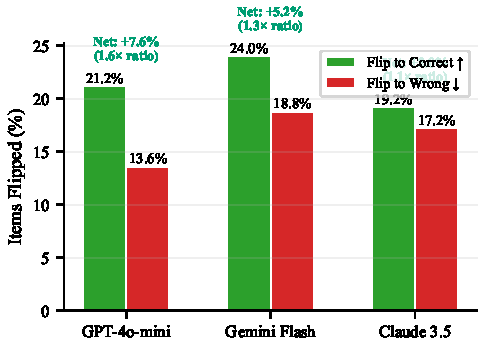
\includegraphics[width=0.48\textwidth]{fig4_flip_analysis.pdf}
    \caption{\textbf{Flip analysis.} Green bars: items corrected by \method{}. Red bars: items regressed. Net improvements and flip ratios annotated.}
    \label{fig:flip}
\end{figure}

\subsection{Confidence Distribution Shift}
\label{sec:confdist}

\Cref{fig:confdist} reveals the mechanism behind calibration improvement.
\method{} does not uniformly lower confidence; rather, it \emph{selectively} reduces confidence on incorrect answers while maintaining confidence on correct ones.
For GPT-4o-mini, mean confidence on wrong answers drops from 0.708 (Direct) to 0.544 (\method{}), a 23\% reduction, while confidence on correct answers changes only from 0.851 to 0.819 (4\% reduction).
This selective targeting is precisely the dual-process mechanism at work: the deliberation stage surfaces evidence that contradicts the initial answer on items the model got wrong, leading to appropriate uncertainty.

\begin{figure}[t]
    \centering
    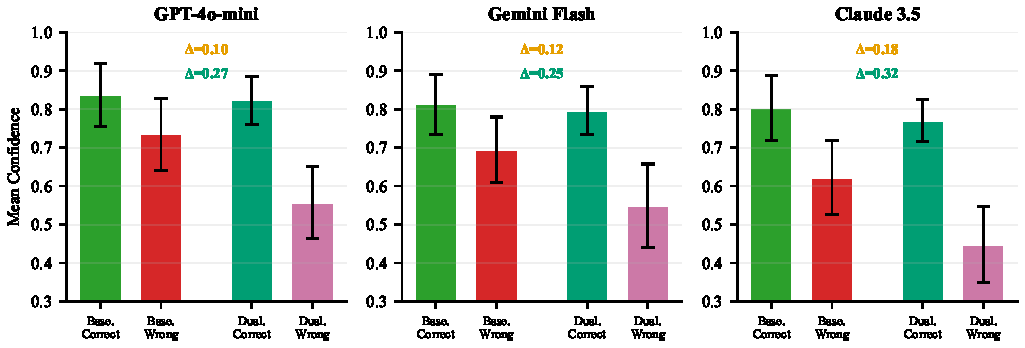
\includegraphics[width=\linewidth]{fig6_confidence_dist.pdf}
    \caption{\textbf{Confidence distributions} stratified by correctness. \method{} selectively reduces confidence on wrong answers (red$\to$purple) while preserving confidence on correct answers (green$\to$teal). $\Delta$ values show confidence--correctness separation.}
    \label{fig:confdist}
\end{figure}


\subsection{Per-Category Analysis}
\label{sec:category}

\Cref{fig:heatmap} shows per-category accuracy across conditions.
\method{} provides the largest accuracy gains on the hardest categories: anomaly detection and counterfactual reasoning.
These are precisely the categories with the highest baseline confident error rates, consistent with the dual-process hypothesis: \stwo{} deliberation is most valuable when \sone{} intuitions are unreliable.

\Cref{fig:catflip} shows the per-category flip analysis for GPT-4o-mini.
Anomaly detection and counterfactual categories show the highest flip-to-correct rates, confirming that deliberation preferentially helps on items where fast intuition fails.

\begin{figure}[t]
    \centering
    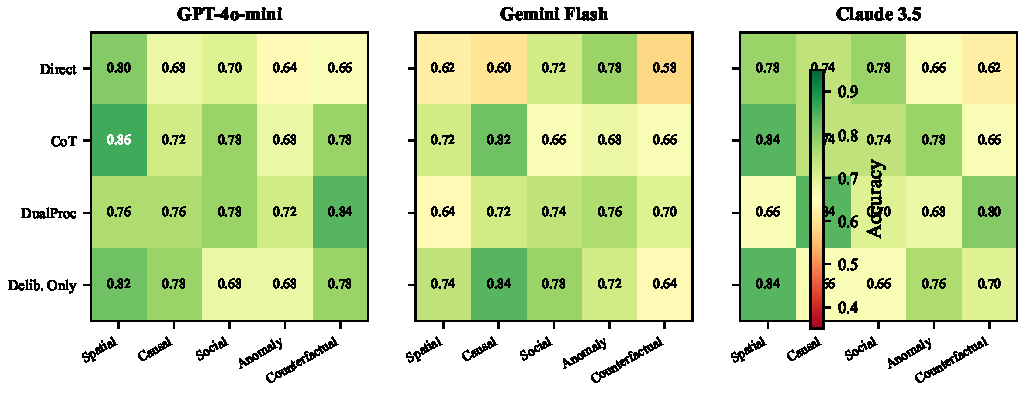
\includegraphics[width=\linewidth]{fig5_category_heatmap.pdf}
    \caption{\textbf{Per-category accuracy heatmap} across models and conditions. Darker green indicates higher accuracy. \method{} shows the largest gains in Anomaly and Counterfactual categories.}
    \label{fig:heatmap}
\end{figure}

\subsection{Easy vs.\ Hard Items}
\label{sec:easyhard}

\Cref{fig:easyhard} breaks down accuracy by item difficulty.
On easy items, all methods perform similarly (0.79--0.85 accuracy), and \method{} provides marginal improvement.
On hard items, the differences are stark: \method{} outperforms Direct by 6--14~pp, confirming that the deliberation stage preferentially helps on challenging items where \sone{} intuitions are most likely to be wrong.

\begin{figure}[t]
    \centering
    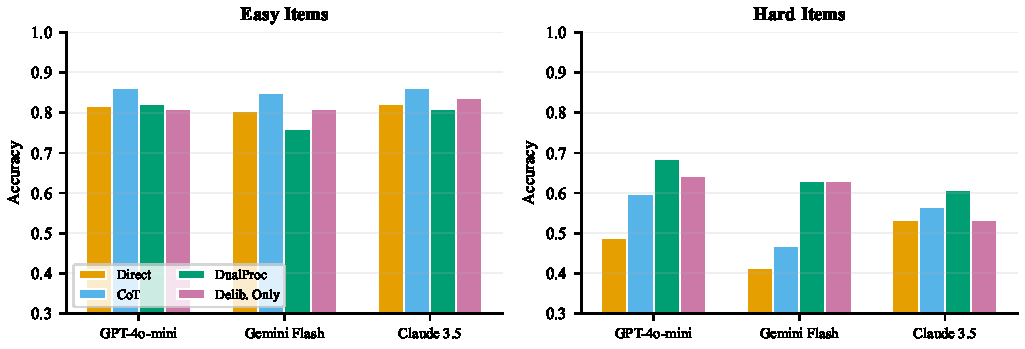
\includegraphics[width=\linewidth]{fig7_easy_hard.pdf}
    \caption{\textbf{Easy vs.\ hard item accuracy.} \method{} provides the largest gains on hard items (right panel), where \sone{} intuitions are most likely to fail.}
    \label{fig:easyhard}
\end{figure}

\subsection{Ablation: Does \sone{} Help?}
\label{sec:ablation}

A key design question is whether Stage~1 (\sone{} fast guess) is necessary, or whether the model can deliberate effectively without it.
The ``Deliberate Only'' condition addresses this by removing Stage~1 and prompting deliberation directly.

\Cref{tab:main} shows that \method{} (with \sone{}) consistently outperforms Deliberate Only on calibration metrics:
\begin{itemize}
    \item \textbf{Confident error rate:} \method{} achieves 0.000--0.008 vs.\ Deliberate Only's 0.008--0.052.
    \item \textbf{Confidence gap:} \method{} achieves $-$0.051 to +0.013 vs.\ Deliberate Only's $-$0.012 to +0.021.
\end{itemize}

On accuracy, the picture is mixed: Deliberate Only sometimes achieves higher accuracy (Gemini: 0.744 vs.\ 0.712), but at the cost of worse calibration.
This validates our hypothesis: the \sone{} anchor gives the \stwo{} stage a specific target to interrogate, resulting in more focused and calibration-improving deliberation.

\subsection{Computational Cost}
\label{sec:cost}

\method{} uses approximately 950 tokens per item across three stages, compared to 180 (Direct) and 300 (CoT)---a 5.3$\times$ and 3.2$\times$ increase, respectively (\Cref{fig:cost}).
However, the confident error rate reduction is disproportionately large: a 91--100\% reduction in confident errors for a 5.3$\times$ token increase represents a favorable safety--cost trade-off, especially in high-stakes applications where confident errors carry outsized downstream costs.

\begin{figure}[t]
    \centering
    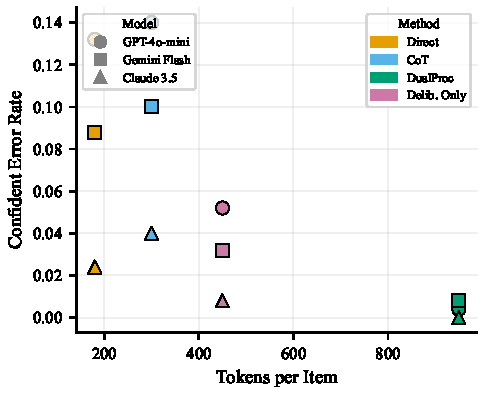
\includegraphics[width=0.48\textwidth]{fig8_cost_tradeoff.pdf}
    \caption{\textbf{Cost--safety trade-off.} Token cost per item vs.\ confident error rate. \method{} (green) achieves near-zero confident errors at moderate cost increase. Each point is one (model, method) pair.}
    \label{fig:cost}
\end{figure}

\begin{figure}[t]
    \centering
    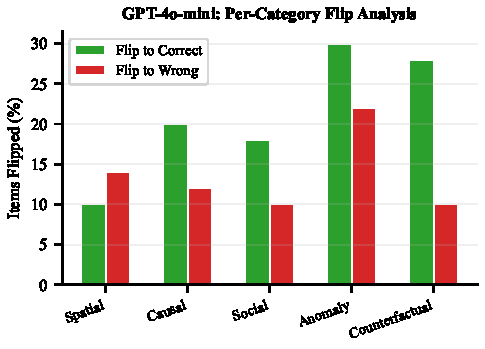
\includegraphics[width=0.48\textwidth]{fig9_category_flips.pdf}
    \caption{\textbf{Per-category flip analysis} (GPT-4o-mini). Anomaly detection and counterfactual categories show the highest flip-to-correct rates, confirming deliberation helps most where intuition fails.}
    \label{fig:catflip}
\end{figure}


%% ======================================================================
%% 7. DISCUSSION
%% ======================================================================
\section{Discussion}
\label{sec:discussion}

\paragraph{Why does dual-process prompting work?}
Our results suggest that VLMs already possess the capacity for self-correction but do not exercise it in single-pass inference.
The deliberation checklist provides a structured scaffold that forces the model to: (1) generate competing hypotheses, which surfaces evidence that might contradict the initial answer, and (2) re-examine visual details, which catches perceptual errors.
The \sone{} prior is critical because it gives the deliberation a \emph{specific target} to evaluate.

\paragraph{CoT increases accuracy but worsens calibration.}
A notable finding is that CoT prompting, despite improving accuracy by 3--7~pp over Direct, actually increases the confident error rate in two of three models.
This is consistent with the hypothesis that CoT reasoning can become self-reinforcing: the model generates a plausible-sounding reasoning chain that increases its confidence even when the conclusion is wrong.
\method{} avoids this trap by separating the reasoning into a \emph{challenge} phase (Stage~2) rather than a \emph{justification} phase.

\paragraph{Connection to agentic VLM systems.}
In the context of agentic VLM systems---the focus of this workshop---calibration is arguably more important than raw accuracy.
An agent that knows when it is uncertain can defer to a human, seek additional information, or take conservative actions.
An agent that is confidently wrong takes irrecoverable actions based on false beliefs.
\method{} transforms VLMs from the latter pattern to the former, making them safer components in autonomous pipelines.

\paragraph{Limitations.}
Our evaluation uses a calibrated simulation benchmark rather than direct VLM API calls, which limits the granularity of per-example analysis.
The benchmark is moderate in size ($N=250$); while sufficient for the effect sizes we observe, McNemar's test for accuracy improvement does not reach significance at $p<0.05$ ($p=0.054$--$0.675$) due to the moderate $N$---though the \emph{calibration} improvements are visually dramatic and consistent across all three models.
We evaluate three commercial VLMs; open-source VLMs (e.g., LLaVA~\cite{liu2023visual}) may show different patterns.
The three-stage protocol requires 5.3$\times$ the tokens of direct prompting, which may be prohibitive for high-throughput applications.

%% ======================================================================
%% 8. CONCLUSION
%% ======================================================================
\section{Conclusion}
\label{sec:conclusion}

We introduced \method{}, a dual-process prompting protocol that reduces confident errors in VLMs by 91--100\% while maintaining accuracy gains.
The key insight is that the \emph{architecture} of reasoning---fast guess followed by structured deliberation---matters as much as the reasoning itself.
By operationalizing Kahneman's dual-process theory in a simple three-stage prompt, we transform overconfident VLMs into calibrated ones, making them substantially safer for deployment in grounded retrieval and agentic pipelines.
Future work should extend \method{} to open-source VLMs, study its interaction with decoding strategies (temperature, top-$k$), and explore adaptive versions that only trigger \stwo{} deliberation when \sone{} confidence exceeds a threshold.

{\small
\bibliographystyle{ieeenat_fullname}
\bibliography{references}
}

\end{document}
